% LaTeX dokumentu guztiak zein dokumentu mota den adieraziz hasi behar dira
\documentclass[es]{ifirak}

% ERABILIKO DIREN PAKETEAK %

% listings paketea kodea formateatzeko erabiltzen da
\usepackage{listings}
% Paquete para los acentos
\usepackage[utf8]{inputenc}

% Paketea konfiguratu behar dugu C lengoaiarekin erabiltzeko:
\definecolor{darkgreen}{rgb}{0,0.5,0}
\definecolor{lightgray}{rgb}{0.95,0.95,0.95}
\definecolor{gray}{rgb}{0.65,0.85,0.45}
\definecolor{white}{rgb}{1,1,1}
\definecolor{purple}{rgb}{0.51,0,0.25}
\definecolor{orange}{rgb}{0.255,0.178,0.102}

\lstdefinestyle{customc}{
	belowcaptionskip=1\baselineskip,
	breaklines=true,
	tabsize=4,
	language=C,
	showstringspaces=false,
	basicstyle=\footnotesize\ttfamily,
	keywordstyle=\bfseries\color{darkgreen},
	commentstyle=\itshape\color{purple},
	identifierstyle=\color{blue},
	stringstyle=\color{orange},
	backgroundcolor=\color{white},
}
\lstset{language=C++,escapechar=@,style=customc}

%\lstset{language=C++,
	%	basicstyle=\scriptsize\ttfamily,
	%	keywordstyle=\color{darkgreen}\bfseries,
	%	identifierstyle=\color{black},
	%	commentstyle=\color{gray}, 
	%	stringstyle=\ttfamily,
	%	showstringspaces=false,
	%	tabsize=2,
	%	backgroundcolor=\color{lightgray}}
%

\begin{document}
% Hainbat datu ...
\ikasturtea{2014 - 2015}
\irakasgaia{Diseño de algoritmos}
% Titulua
\title{Práctica de Programación 1}
% Zuen izena
\author{Mikel Dalmau}

\maketitle

% Abstract ingurunea hasierako laburpena idazteko erabili
\begin{abstract}
En la siguiente práctica se realiza un estudio analítico y experimental de varias de las distintas soluciones para el problema de hallar un segmento de suma máxima en una secuencia de enteros.
\end{abstract}

% Testua egituratzeko section, subsection, subsubsection, subsubsection eta paragraph komandoak dituzue
\section{Solución cúbica}
\paragraph{}
La siguiente solución explora todos los segmentos posibles de la secuencia, realiza una nueva suma para cada segmento y compara dicho valor con el maximo alcanzado hasta el momento. 
\subsection{Estudio analítico}
\paragraph{}
El código del algoritmo es el siguiente:
\begin{lstlisting}
void segSumaMaxH(string fname){
	vector<int> V;
	int n,i,j,k,sum,maxSum,start,end;
	
	leerFichero(fname, &V, &n);
	maxSum = V[0]; start = 0; end = 0;
	for(i = 0; i < n ; i++){
		for(j = i; j < n ; j++){
			sum = 0;
			for(k = i; k < j +1; k++){
				sum = sum + V.at(k);
				if( sum > maxSum){
					maxSum = sum;
					start = i;
					end = j;
				}
			}
		}
	}
	cout << start << " " << end - 1 << " " << maxSum << endl; 
};
\end{lstlisting}
\paragraph{}
Observando el código podemos ver que realiza 3 bucles y un acceso al vector por cada iteración del bucle de mas al interior, el resto de operaciones son de orden constante, y el acceso al vector es también de complejidad constante \cite{key-1}. La función de coste de este algoritmo es entonces de la siguiente forma:


$$f(n)= \sum_{i=1}^{n}\sum_{j=1}^{n}\sum_{k=i}^{j} 1 $$
$$f(n)=\sum_{i=1}^{n}\sum_{j=1}^{n}(j-i+1)
 =\sum_{i=1}^{n}(1+2+...+(n-i+1))
 =\sum_{k=1}^{n}k + \sum_{k=1}^{n-1}k + ... + \sum_{k=1}^{1}k=$$
$$ = \frac{(n+1)n}{2} + \frac{(n-1)n}{2} + \frac{(n+1)(n-2)}{2} +...+ \frac{2\times1}{2}=$$
$$=\frac{1}{2}\sum_{k=1}^{n}k(k+1)
=f(n-1)+\frac{(n+1)n}{2}
=\frac{(n+2)(n+1)n}{6} \equiv O(n^{3})$$
\paragraph{}
Vemos que finalmente la solución resulta ser de orden cúbico y ya podía intuirse por el hecho de contener 3 bucles uno dentro de otro.
\subsection{Estudio experimental}

\paragraph{}
El lenguaje de programación utilizado para las pruebas de los algoritmos ha sido c++, la computadora es una HP pavilion dv7 con procesador AMD 2.8 Ghz y arquitectura de 64 bits.
\paragraph{}
El tamaño de las pruebas realizadas con cada algoritmo varía dependiendo del tiempo de computo de cada uno, de forma que hubiera suficientes datos para distinguir el orden de crecimiento y se terminaran en un tiempo razonable.
\paragraph{}
Para indicar el tamaño de entrada se ha utilizado la siguiente notación (1000 enteros = 1K). Se ha realizado tres pruebas para cada algoritmo con tamaños iguales pero entradas distintas en cada una, luego se ha realizado una media de las pruebas.

\paragraph{}
\begin{center}
	\begin{table}[htbp]
		\centering
		\begin{tabular}{c|c|c|c|c|c}
			N (K) & T(s) Prueba1 & T(s) Prueba2 & T(s) Prueba3 & media & $\sqrt[3]{media}$\\
			\hline
			1 & 3.51 & 3.167 & 3.213 & 3.297 & 1.488\\
			2 & 27.55 & 25.975 & 24.227 & 25.917 & 2.959\\
			4 & 218.027 & 198.527 & 205.672 & 207.408 & 5.919\\
			8 & 1732.55 & 1684.421 & 1761.954 & 1726.308 & 11.995\\
			10 & 3410.31  & 3280.897 & 3457.159 & 3382.788 & 15.012\\
		\end{tabular}
		\caption{Tiempos solución cúbica.}\label{table}
	\end{table}
\end{center}
\paragraph{}
En las siguientes gráficas podemos apreciar el crecimiento cuadrático del tiempo de cómputo, y como al hacer la raíz de estos valores la función se hace lineal.
\begin{figure}[htbp]
	\centering
	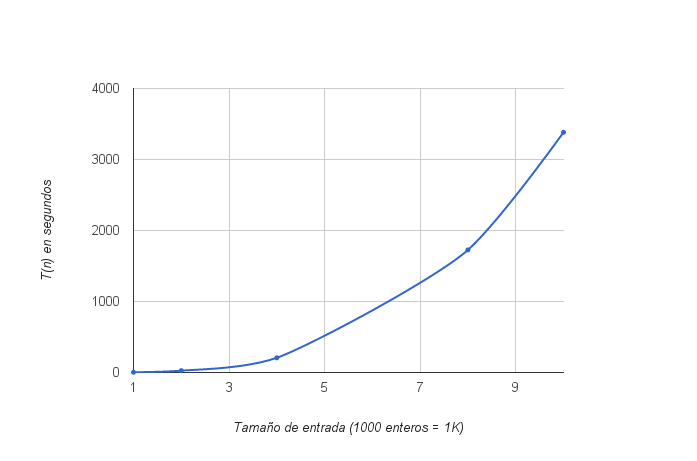
\includegraphics[width=0.8\textwidth]{cubica.png}
	\caption{Representación gráfica de los datos de la tabla 1.}\label{figure}
\end{figure}

\begin{figure}[htbp]
	\centering
	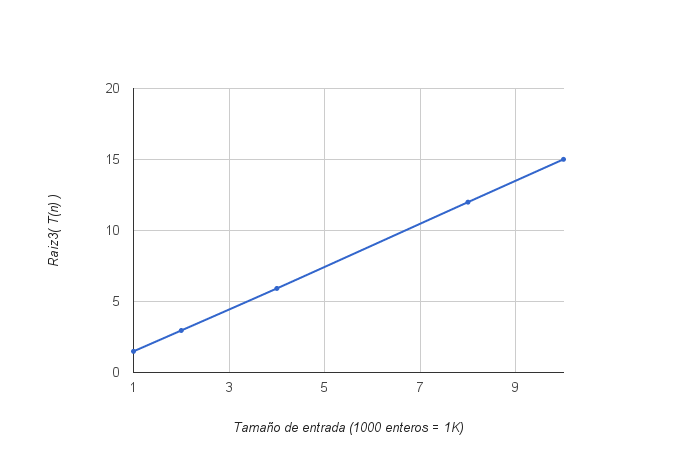
\includegraphics[width=0.8\textwidth]{raiz3.png}
	\caption{Representación gráfica de los datos de la tabla 1.}\label{figure}
\end{figure}
\newpage
\section{Solución cuadrática}
\paragraph{}
La siguiente solución explora todos los segmentos posibles de la secuencia y es similar a la anterior solo que utiliza el calculo de la suma del anterior segmento para el siguiente ahorrando uno de los bucles.
\subsection{Estudio analítico}

\paragraph{}
El código del algoritmo es el siguiente:
\begin{lstlisting}
void segSumaMaxF(string fname){
	vector<int> V;
	int n,i,j,sum,maxSum,start,end;
	
	leerFichero(fname, &V, &n);
	maxSum = V[0]; start = 0; end = 0;
	for(i = 0; i < n ; i++){
		sum = 0;
		for(j = i; j < n ; j++){
			sum = sum + V.at(j);
			if( sum > maxSum){
				maxSum = sum;
				start = i;
				end = j;
			}
		}
	}
	cout << start << " " << end << " " << maxSum << endl;
};
\end{lstlisting}
\paragraph{}
El código es idéntico al anterior con la salvedad de ese tercer bucle que ahorra, la función de coste sería la siguiente.
$$g(n)= \sum_{i=1}^{n}\sum_{j=1}^{n} 1 $$
$$g(n)=\sum_{i=1}^{n}n = n^{2} \equiv O(n^{2})$$
\subsection{Estudio experimental}
\paragraph{}
\begin{table}[htbp]
	\centering
	\begin{tabular}{c|c|c|c|c|c}
		N (K) & T(s) Prueba1 & T(s) Prueba2 & T(s) Prueba3 & media & $\sqrt{media}$\\
		\hline
		4 & 0.218& 0.14 & 0.156& 0.171 & 0.414\\
		16 & 2.45 & 2.434& 2.371& 2.418  &	1.555\\
		64 & 41.636 & 38.609& 36.817& 39.0206 &	6.246\\
		100 & 104.225  & 95.879& 91.573& 97.225	& 9.860\\
		200 &  411.21 & 388.643& 421.824& 407.225 & 	20.179\\
	\end{tabular}
	\caption{Tiempos solución cuadrática.}\label{table}
\end{table}

\begin{figure}[htbp]
	\centering
	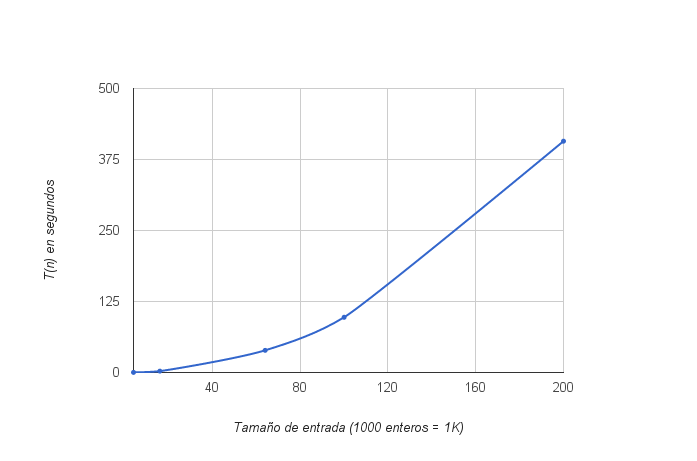
\includegraphics[width=0.8\textwidth]{cuadratica.png}
	\caption{Representación gráfica de los datos de la tabla 2.}\label{figure}
\end{figure}

\begin{figure}[htbp]
	\centering
	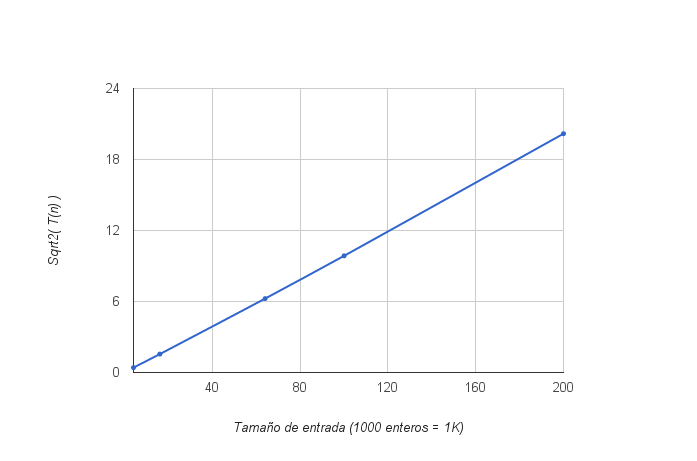
\includegraphics[width=0.8\textwidth]{raiz2.png}
	\caption{Representación gráfica de los datos de la tabla 2.}\label{figure}
\end{figure}
\newpage


\section{Solución recursiva, divide y vencerás}
La siguiente solución es mas enrevesada que las anteriores pero su orden mejora considerablemente tal y como comprobaremos más adelante.
\subsection{Estudio analítico}

\paragraph{}
Este algoritmo divide la tabla en dos mitades que resuelve recursivamente, después realiza la tarea adicional de calcular cual es el segmento de suma máxima que necesariamente incluya elementos de ambas mitades. Esta tarea se realiza con la función sumaMaxCentro que estudia todos los segmentos que terminan o comienzan en un índice central y posteriormente los une.
\paragraph{}
El código del algoritmo es el siguiente:
\begin{lstlisting}
sumAndIndex segSumaMaxR(vector<int> *v,int i, int j){
	sumAndIndex eI,eD,eC,e;
	int i, j;
	int mid = i + (j-i)/2;
	
	if(not (i != j)){
		e.sum=v->at(i); e.i=i; e.j=i;
		return e;
	}else{
		eI = segSumaMaxR(v,i,mid);
		eD = segSumaMaxR(v,mid+1,j);
		eC = sumMaxCentro(v,i,j,mid);
	}
	if ((eD.sum <= eI.sum) and (eC.sum <= eI.sum)){
		return eI;
	}
	if ((eI.sum <= eD.sum) and (eC.sum <= eD.sum)){
		return eD;
	}
	if ((eI.sum <= eC.sum) and (eD.sum <= eC.sum)){
		return eC;
	}
};
/*
*
*/
sumAndIndex sumMaxCentro(vector<int> *v,int i, int j,int centro){
	int k,partial,maxI,maxD,auxI,auxD;
	sumAndIndex e;
	int i, j;
	
	maxI = v->at(centro); auxI = centro; partial = v->at(centro);
	for(k = centro-1; k > i-1; k--){
		partial = partial + v->at(k);
		if(partial > maxI){
			maxI = partial;
			auxI = k;
		}
	}
	maxD = v->at(centro+1); auxD = centro + 1; partial = v->at(centro+1);
	for(k = centro+2; k < j+1; k++){
		partial = partial + v->at(k);
		if(partial > maxD){
			maxD = partial;
			auxD = k;
		}
	}
	e.i = auxI; e.j = auxD; e.sum = maxI + maxD;
	return e;
};
\end{lstlisting}
\paragraph{}
La función de coste será de la siguiente forma:
$$T(n)=2T(\frac{n}{2}) + \Theta(n)$$
Sabemos que el coste de juntar las partes del problema es lineal en n pues el subprograma sumMaxCentro recorre la lista de elementos desde el centro hacia la izquierda y hacia la derecha y como máximo recorrerá n elementos.

\paragraph{}
Podemos hallar fácilmente el orden de la expresión recursiva.

$$T(n)=2T(\frac{n}{2}) + n = 2(2T(\frac{n}{4}) + \frac{n}{2})+n = 2^{i}T( \frac{n}{2^{i}}) + in$$


$$Caso \hspace{0.2cm} base: \hspace{0.5cm} \frac{n}{2^{i}} = 1 \rightarrow i = \lg n$$

$$2^{\lg n}T(\frac{n}{2^{\lg n}}) + ( \lg n)n = 2^{\lg n}T(\frac{n}{n}) + (\lg n)n = n + n \lg n \equiv O(n \lg n) $$

$$ \omega(n) \equiv  O(n \lg n) \equiv o(n^{2})  $$
Vemos que el orden ahora ha mejorado considerablemente respecto del cuadrático pero no llega a ser lineal todavía.
\subsection{Estudio experimental}
\paragraph{}
\begin{table}[htbp]
	\centering
	\begin{tabular}{c|c|c|c|c}
		N (K) & T(s) Prueba1 & T(s) Prueba2 & T(s) Prueba3 & media  \\
		\hline
		32 & 0.016 & 0.016& 0.015 & 0.0157  \\
		100 & 0.062 & 0.078 & 0.063& 0.068 \\
		200 & 0.109 & 0.125 & 0.094 & 0.109 \\
		500 & 0.343 & 0.358 & 0.311 & 0.337 \\
		1000 & 0.624 & 0.687 & 0.577 & 0.6293\\
	\end{tabular}
	\caption{Tiempos solución recursiva.}\label{table}
\end{table}

\paragraph{}
Como podemos ver en la siguiente gráfica no se distingue mucho de la lineal, probablemente sean necesarias entradas mayores a 1 millon para apreciar el crecimiento de la curva.
\newpage
\begin{figure}[htbp]
	\centering
	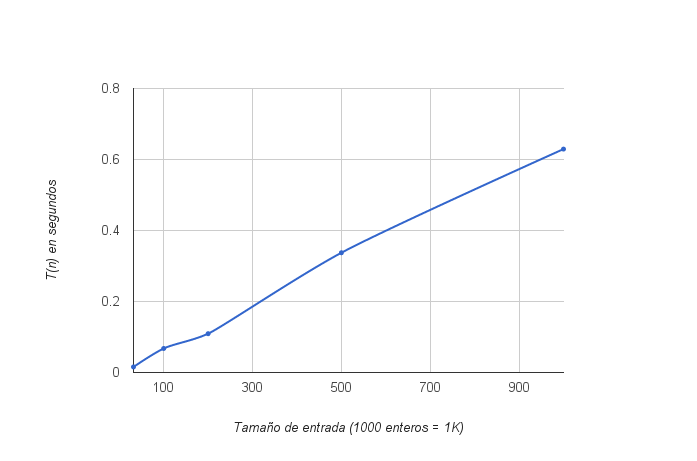
\includegraphics[width=0.8\textwidth]{logaritmica.png}
	\caption{Representación gráfica de los datos de la tabla 3.}\label{figure}
\end{figure}

\newpage
\section{Solución lineal}
\subsection{Estudio analítico}
\paragraph{}
El algoritmo de Kadane consiste en recorrer el array de elementos calculando la suma positiva máxima en cada posición, si se alcanza una posición de valor negativo o dicho de otra forma, la suma acumulada decrece, entonces comenzamos a contar otra vez. Este subarray puede ser o vacío en cuyo caso la suma será cero o puede contener un elemento más que el subarray maximo que terminaba en la posición anterior.\cite{key-2}

\paragraph{}
Uno de los problemas de este algoritmo es que falla cuando la entrada son todo números negativos es por eso que he incluido en el código un par de valores que almacenen el elemento de mayor valor de toda la lista y su posición, en caso de que este elemento sea negativo entonces la solución es dicho elemento.
\paragraph{}
El código del algoritmo es el siguiente:
\begin{lstlisting}
void Kadane(string fname){
	vector<int> v;
	int max, max_temp, n, start, end, max_start, max_end,val_temp,max_special,pos_special;
	leerFichero(fname, &v, &n) < 0)
	
	max_temp = v.at(0); max = max_temp; start = 0; end = 0; max_start = 0; max_end = 0; max_special = v.at(0); pos_special = 0;
	for (int i = 1; i < n; i++){
		val_temp =  v.at(i);
		if(val_temp > max_special){
			max_special  = val_temp;
			pos_special = i;
		}
		if( val_temp >  (max_temp + val_temp)){
			start = i;
			end = i;
			max_temp =  val_temp;
		}else{
			end = i;
			max_temp = max_temp + val_temp;
		}
		if(max_temp > max){
			max = max_temp;
			max_start = start;
			max_end = end;
		}
	}
	if(max_special < 0){
		cout << pos_special << " " << pos_special << " " << max_special << endl; 
	}else{
		cout << max_start << " " << max_end << " " << max << endl; 
	}
};
\end{lstlisting}
\paragraph{}
Con un vistazo al código podemos ver que sólo incluye un bucle que recorre los n elementos y una serie de comparaciones y asignaciones y un acceso al vector que como vimos es de orden lineal. Por esto la función de coste del algoritmo será la siguiente.

$$f(n)= \sum_{i=1}^{n} O(1) \equiv O(n)$$

\newpage
\subsection{Estudio experimental}
\paragraph{}
\begin{center}
	\begin{table}[htbp]
		\centering
		\begin{tabular}{c|c|c|c|c}
			N (K) & T(s) Prueba1 & T(s) Prueba2 & T(s) Prueba3 & media \\
			\hline
		100 &	0.015&	0.016&	0.015&	0.015\\
		200 & 	0.031&	0.031&	0.047&	0.036\\
		500 &	0.078&	0.093&	0.078&	0.083\\
		750 &	0.11&	0.125&	0.203&	0.146\\
		1000 & 	0.202&	0.187&	0.187&	0.192\\
		
		\end{tabular}
		\caption{Tiempos solución lineal.}\label{table}
	\end{table}
\end{center}

\paragraph{}
Podemos en la gráfica de los tiempo de ejecución que se asemeja bastante a una línea recta.

\begin{figure}[htbp]
	\centering
	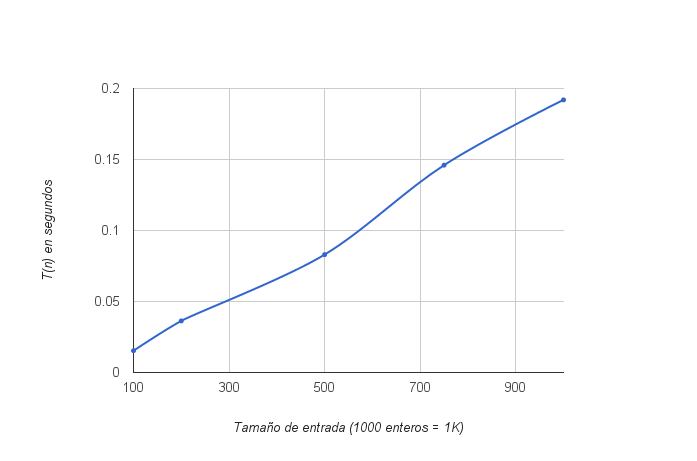
\includegraphics[width=0.8\textwidth]{KadaneGrafica.png}
	\caption{Representación gráfica de los datos de la tabla 4.}\label{figure}
\end{figure}



\newpage
\begin{thebibliography}{arauak}
	
	\bibitem[cppRef]{key-1} http://es.cppreference.com .
	
	\bibitem[Wiki]{key-2} http://en.wikipedia.org/wiki/Maximum\_subarray\_problem .
	
	\bibitem[Sedge]{key-3} Algorithms 4th edition Sedgewick \& Wayne, Pearson
	
\end{thebibliography}


\section{Anéxo}
\paragraph{Comentarios:}
Han surgido algunos problemas de última hora en la representación de los resultados así como en el tiempo de ejecución. En algunos casos he obtenido indices i negativos como solución, no he hallado el error que lo causa, pero les ha sucedido a varios de los algoritmos, de todas formas las soluciones son iguales en todos los algoritmos.\\
También debido a algunos cambios que sin duda están relacionados con lo anterior he notado  diferencias significativas en el tiempo de cómputo de los algoritmos cuadrático y cúbico. En cualquier caso se puede apreciar como escala el tiempo sin ningún problema pero es posible que sea necesario corregir algún pequeño matiz que no he podido encontrar.
\paragraph{}
Las siguientes páginas contienen todo el código utilizado, en lenguaje c++.
\begin{lstlisting}
/* 
* File:   main.cpp
* Author: mdalmau002
*
* Created on 8 de marzo de 2015, 12:35
*/
#include <vector>
#include <cstdlib>
#include <algorithm>
#include <iostream>
#include <fstream>
#include <cmath>
#include <time.h>
using namespace std;

//Estrucutra utilizada para devolver los tres datos en el algoritmo recursivo
typedef struct {
	int i;
	int j;
	int sum;
} sumAndIndex;

void crearBloquePruebas();
void crearFicheroPrueba(int size , string name);
int leerFichero(string fname, vector<int> *pV, int *n);
void segSumaMaxH(string fname);
void segSumaMaxF(string fname);
sumAndIndex sumMaxCentro(vector<int> *v,int pi, int pj,int centro);
sumAndIndex segSumaMaxR(vector<int> *v,int pi, int pj);
void segSumaMaxRecursivo(string fname);
void Kadane(string fname);
void ejecutarBloqueKadane();
void ejecutarBloqueR();
void ejecutarBloqueH();
void ejecutarBloqueF();

int main ()
{
	crearBloquePruebas();
	ejecutarBloqueKadane();
	ejecutarBloqueR();
	ejecutarBloqueF();
	ejecutarBloqueH();
	return 0;
}
/*
*
*/
void Kadane(string fname){
	vector<int> v;
	int max, max_temp, n, start, end, max_start, max_end,val_temp,max_special,pos_special;
	leerFichero(fname, &v, &n) < 0)
	
	max_temp = v.at(0); max = max_temp; start = 0; end = 0; max_start = 0; max_end = 0; max_special = v.at(0); pos_special = 0;
	for (int i = 1; i < n; i++){
		val_temp =  v.at(i);
		if(val_temp > max_special){
			max_special  = val_temp;
			pos_special = i;
		}
		if( val_temp >  (max_temp + val_temp)){
			start = i;
			end = i;
			max_temp =  val_temp;
		}else{
			end = i;
			max_temp = max_temp + val_temp;
		}
		if(max_temp > max){
			max = max_temp;
			max_start = start;
			max_end = end;
		}
	}
	if(max_special < 0){
		cout << pos_special << " " << pos_special << " " << max_special << endl; 
	}else{
		cout << max_start << " " << max_end << " " << max << endl; 
	}
};
/*
*
*/
void segSumaMaxRecursivo(string fname){
	vector<int> V;
	int n;
	sumAndIndex sol;
	
	leerFichero(fname, &V, &n) < 0)
	sol = segSumaMaxR(&V, 0, n-1);
	cout << sol.i << " " << sol.j << " " << sol.sum << endl; 
};
/*
*
*/
sumAndIndex segSumaMaxR(vector<int> *v,int pi, int pj){
	sumAndIndex eI,eD,eC,e;
	int i, j;
	i = pi; j = pj;
	int mid = i + (j-i)/2;
	
	if(not (i != j)){
		e.sum=v->at(i); e.i=i; e.j=i;
		return e;
	}else{
		eI = segSumaMaxR(v,i,mid);
		eD = segSumaMaxR(v,mid+1,j);
		eC = sumMaxCentro(v,i,j,mid);
	}
	if ((eD.sum <= eI.sum) and (eC.sum <= eI.sum)){
		return eI;
	}
	if ((eI.sum <= eD.sum) and (eC.sum <= eD.sum)){
		return eD;
	}
	if ((eI.sum <= eC.sum) and (eD.sum <= eC.sum)){
		return eC;
	}
};
/*
*
*/
sumAndIndex sumMaxCentro(vector<int> *v,int pi, int pj,int centro){
	int k,partial,maxI,maxD,auxI,auxD;
	sumAndIndex e;
	int i, j;
	i = pi; j = pj;
	
	maxI = v->at(centro); auxI = centro; partial = v->at(centro);
	for(k = centro-1; k > i-1; k--){
		partial = partial + v->at(k);
		if(partial > maxI){
			maxI = partial;
			auxI = k;
		}
	}
	maxD = v->at(centro+1); auxD = centro + 1; partial = v->at(centro+1);
	for(k = centro+2; k < j+1; k++){
		partial = partial + v->at(k);
		if(partial > maxD){
			maxD = partial;
			auxD = k;
		}
	}
	e.i = auxI; e.j = auxD; e.sum = maxI + maxD;
	return e;
};
/*
*
*/
void segSumaMaxF(string fname){
	vector<int> V;
	int n,i,j,sum,maxSum,start,end;

	leerFichero(fname, &V, &n);
	maxSum = V[0]; start = 0; end = 0;
	for(i = 0; i < n ; i++){
		sum = 0;
		for(j = i; j < n ; j++){
			sum = sum + V.at(j);
			if( sum > maxSum){
				maxSum = sum;
				start = i;
				end = j;
			}
		}
	}
	cout << start << " " << end << " " << maxSum << endl;
};
/*
*
*/
void segSumaMaxH(string fname){
	vector<int> V;
	int n,i,j,k,sum,maxSum,start,end;
	
	leerFichero(fname, &V, &n);
	maxSum = V[0]; start = 0; end = 0;
	for(i = 0; i < n ; i++){
		for(j = i; j < n ; j++){
			sum = 0;
			for(k = i; k < j +1; k++){
				sum = sum + V.at(k);
				if( sum > maxSum){
					maxSum = sum;
					start = i;
					end = j;
				}
			}
		}
	}
	cout << start << " " << end - 1 << " " << maxSum << endl; 
};
/* 
* Input: Nombre de fichero y apuntador a array de enteros y tamano del array
* Outpu: Rellena array de enteros con los datos del fichero
*/
int leerFichero(string fname, vector<int> *pV, int *n){
	int i,lines;
	ifstream fe(fname.c_str());
	
	fe >> lines;
	*n = lines;
	if(not(lines > 1000000 or lines < 1)){
		vector<int> V(lines);
		for(i = 0; i < lines ; i++){
			fe >> V.at(i);
		}
		cout << V.back();
		*pV = V;
		fe.close();
		return 0;
	}
	fe.close();
	return -1;
};
/* 
* Input: int size, tamano de la lista de elementos, fname nombre para el fichero
* Output: Construye un fichero con un entero positivo en la primera linea indicando el numero de lineas
*  que contiene el fichero
*/
void crearFicheroPrueba(int size , string fname){
	int i,num;
	ofstream fs(fname.c_str());
	
	fs << size << endl;
	for (i = 0; i < size ; i++ ){     
		num = (rand() % 201) - 100;
		fs << num << endl;
	}
	fs.close();
};
/*
* Construye un bloque de ficheros de distintos tamanos para realizar las pruebas
*/
void crearBloquePruebas(){
	crearFicheroPrueba(1000,"1Ksec.txt");
	crearFicheroPrueba(2000,"2Ksec.txt");
	crearFicheroPrueba(4000,"4Ksec.txt");
	crearFicheroPrueba(5000,"5Ksec.txt");
	crearFicheroPrueba(8000,"8Ksec.txt");
	crearFicheroPrueba(16000,"16Ksec.txt");
	crearFicheroPrueba(10000,"10Ksec.txt");
	crearFicheroPrueba(32000,"32Ksec.txt");
	crearFicheroPrueba(64000,"64Ksec.txt");
	crearFicheroPrueba(100000,"100Ksec.txt");
	crearFicheroPrueba(200000,"200Ksec.txt");
	crearFicheroPrueba(500000,"500Ksec.txt");
	crearFicheroPrueba(750000,"750Ksec.txt");
	crearFicheroPrueba(1000000,"1000Ksec.txt");
};
/*
*En los siguientes bloques esta definido como se ejecutan las pruebas y con que ficheros
* 
*/
void ejecutarBloqueKadane(){
	clock_t tic,toc;
	cout << "Lineal" << endl;
	tic = clock();
	Kadane("100Ksec.txt");
	toc = clock();
	cout << "Elapsed 100K: " << ((double)(toc - tic) / CLOCKS_PER_SEC) << " seconds" << endl;
	
	tic = clock();
	Kadane("200Ksec.txt");
	toc = clock();
	cout << "Elapsed 200K: " << ((double)(toc - tic) / CLOCKS_PER_SEC) << " seconds" << endl;
	
	tic = clock();
	Kadane("500Ksec.txt");
	toc = clock();
	cout << "Elapsed 500K: " << ((double)(toc - tic) / CLOCKS_PER_SEC) << " seconds" << endl;
	
	tic = clock();
	Kadane("750Ksec.txt");
	toc = clock();
	cout << "Elapsed 750K: " << ((double)(toc - tic) / CLOCKS_PER_SEC) << " seconds" << endl;
	
	tic = clock();
	Kadane("1000Ksec.txt");
	toc = clock();
	cout << "Elapsed 1000K: " << ((double)(toc - tic) / CLOCKS_PER_SEC) << " seconds" << endl;
};

void ejecutarBloqueH(){

	clock_t tic,toc;
	
	cout << "Cubico" << endl;
	tic = clock();
	segSumaMaxH("1Ksec.txt");
	toc = clock();
	cout << "Elapsed 1K: " << ((double)(toc - tic) / CLOCKS_PER_SEC) << " seconds" << endl;
	
	tic = clock();
	segSumaMaxH("2Ksec.txt");
	toc = clock();
	cout << "Elapsed 2K: " << ((double)(toc - tic) / CLOCKS_PER_SEC) << " seconds" << endl;
	
	tic = clock();
	segSumaMaxH("4Ksec.txt");
	toc = clock();
	cout << "Elapsed 4K: " << ((double)(toc - tic) / CLOCKS_PER_SEC) << " seconds" << endl;
	
	tic = clock();
	segSumaMaxH("8Ksec.txt");
	toc = clock();
	cout << "Elapsed 8K: " << ((double)(toc - tic) / CLOCKS_PER_SEC) << " seconds" << endl;
	
	tic = clock();
	segSumaMaxH("10Ksec.txt");
	toc = clock();
	cout << "Elapsed 10K: " << ((double)(toc - tic) / CLOCKS_PER_SEC) << " seconds" << endl;
};

void ejecutarBloqueF(){
	clock_t tic,toc;
	cout << "Cuadratico" << endl;
	
	tic = clock();
	segSumaMaxF("4Ksec.txt");
	toc = clock();
	cout << "Elapsed 4K: " << ((double)(toc - tic) / CLOCKS_PER_SEC) << " seconds" << endl;
	
	tic = clock();
	segSumaMaxF("16Ksec.txt");
	toc = clock();
	cout << "Elapsed 16K: " << ((double)(toc - tic) / CLOCKS_PER_SEC) << " seconds" << endl;
	
	tic = clock();
	segSumaMaxF("32Ksec.txt");
	toc = clock();
	cout << "Elapsed 32K: " << ((double)(toc - tic) / CLOCKS_PER_SEC) << " seconds" << endl;
	
	tic = clock();
	segSumaMaxF("64Ksec.txt");
	toc = clock();
	cout << "Elapsed 64K: " << ((double)(toc - tic) / CLOCKS_PER_SEC) << " seconds" << endl;
	
	tic = clock();
	segSumaMaxF("100Ksec.txt");
	toc = clock();
	cout << "Elapsed 100K: " << ((double)(toc - tic) / CLOCKS_PER_SEC) << " seconds" << endl;
};

void ejecutarBloqueR(){
	clock_t tic,toc;
	
	tic = clock();
	segSumaMaxRecursivo("32Ksec.txt");
	toc = clock();
	cout << "Elapsed 32K: " << ((double)(toc - tic) / CLOCKS_PER_SEC) << " seconds" << endl;
	
	tic = clock();
	segSumaMaxRecursivo("100Ksec.txt");
	toc = clock();
	cout << "Elapsed 100K: " << ((double)(toc - tic) / CLOCKS_PER_SEC) << " seconds" << endl;
	
	tic = clock();
	segSumaMaxRecursivo("200Ksec.txt");
	toc = clock();
	cout << "Elapsed 200K: " << ((double)(toc - tic) / CLOCKS_PER_SEC) << " seconds" << endl;
	
	tic = clock();
	segSumaMaxRecursivo("500Ksec.txt");
	toc = clock();
	cout << "Elapsed 500K: " << ((double)(toc - tic) / CLOCKS_PER_SEC) << " seconds" << endl;
	
	cout << " n log n" << endl;
	tic = clock();
	segSumaMaxRecursivo("1000Ksec.txt");
	toc = clock();
	cout << "Elapsed 1000K: " << ((double)(toc - tic) / CLOCKS_PER_SEC) << " seconds" << endl;
};
\end{lstlisting}


\end{document}
